%! Author = Tom
%! Date = 07.12.2022
\chapter{Einleitung}

In diesem Kapitel wird an das Thema und die Motivation dieser Arbeit herangeführt.
Außerdem wird definiert, welche Ziele diese Arbeit erreichen soll und eine grobe Übersicht über die
Kapitelstruktur gegeben.

\section{Motivation}

Mit einer steigenden Nutzung von GraphQL wird es immer wichtiger, geeignete Tests für GraphQL-API's zu entwickeln damit eine
gute Softwarequalität sichergestellt werden kann.
Tests können manuell geschrieben oder automatisch generiert werden.
Während bei Unit-Tests für einzelne Methoden der Programmierer frei entscheiden kann, ob er die Tests selbst schreiben will
oder doch eher von einem Tool generieren lassen will sind bei Integrations-Tests die Testräume teilweise so groß, dass ein
manuelles Schreiben dieser Tests einerseits fehleranfällig aber auch schlicht zu langwierig ist.
Für REST-APIs existieren schon automatische Integrationstesttools wie zum Beispiel: EvoMaster \cite{evo-master} , QuickREST \cite{karlsson2019quickrest} oder RESTTESTGEN \cite{rest-test-gen}.
GraphQL-APIs haben leider noch einen Mangel an solchen automatischen Testtools.
Im Rahmen der IEEE/ACM 2021 wurde mit ''Automatic Property-based Testing of GraphQL APIs''\cite{property-based-testing} eine Methode vorgestellt die diesen Mangel angehen soll.
Ergebnis der Arbeit war hierbei ein Prototyp der die vorgestellte Methode umsetzten sollte.
Die vorgestellte Methode bezieht sich auf ''Property-based Testing'' wobei diese gleichzusetzen ist mit ''Random Testing'' \cite{property-based-testing}[vgl. 2.B]
Durch die starke Typisierung und Schema-Definition, welche prinzipiell ein Graph ist, lässt sich in GraphQL
sehr einfach auswerten welche Anfragen nun zulässig sind.
Die hier vorgestellte Methode nutzt den Fakt, dass zum Beispiel alle möglichen Anfragen immer im Query-Knoten
beginnen müssen und somit alle weitergehenden Felder im Schema innerhalb des Query-Knoten definiert sein müssen.
Da die Definition des Schemas der eines Graphens entspricht ist jedoch der mögliche Suchraum potentiell unendlich da GraphQL
Zyklen innerhalb des Graphens erlaubt.
Der unendliche Suchraum wurde durch ein Rekursionslimit begrenzt allerdings wird so eine schlechtere Test-Coverage erreicht.
\newpage
Die bisher entwickelte Methode funktioniert auf folgende Weise:

\begin{center}
    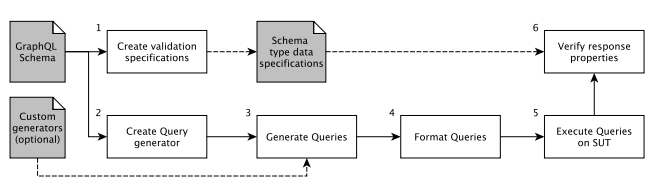
\includegraphics[width=\textwidth,height=\textheight,keepaspectratio]{content/einleitung/toolchain}
    \caption{Methode von~\cite{property-based-testing}}
\end{center}

wobei neben dem vorher erwähnten Rekursionslimit außerdem Punkt 6. ''Verify response Properties'' kritisch
zu betrachten ist da die Auswertung wirklich nur auf die Properties schaut.
Dies bedeutet, dass ein zurückgegebens Objekt nur auf seinen Typ überprüft wird aber nicht, ob seine tatsächlichen Rückgabewerte, die exakt erwartet sind.
Hierdurch können false-positives entstehen.

Die vorgestellte Methode wollen wir verbessern durch Änderung einiger Ansätze.
Hierbei sollen Graphcoverage-Algorithmen zum Einsatz kommen, die mit iterativen Verfahren auch zyklische Graphen ideal
überdecken können und dabei immer verlässlich arbeiten, sodass die generierten Tests stets für vergleichbare Ergebnisse sorgen und nicht
davon abhängig sind, dass der Zufall eine gute Überdeckung liefert.
Zusammenfassend sei gesagt, dass bei der Testgenerierung und Testauswertung Verbesserungen möglich sind und dies Gegenstand dieser Arbeit sein soll.

\section{Umsetzung}

Zuallererst wird in dieser Arbeit etwas Theorie definiert und in Bezug gesetzt.
Wir beginnen damit die Graphentheorie als mathematisches Konzept zu definieren denn dieses liegt GraphQL zugrunde.
Darauffolgend kommt eine kleine Einführung in GraphQL und dann bilden wir schon die Schnittstelle von GraphQL zur Graphentheorie.
Sobald diese Verbindung erfolgt ist können wir uns dem eigentlichen Problem widmen: Wie kann man mithilfe von Graphcoverage-Algorithmen
Tests generieren?
Hierfür erfolgt ein letzter Theorie-Exkurs über Software-Tests.
Mit diesen Grundlagen schaffen wir es dann unsere Methode zu entwickeln und können Sie auch mit ''Automatic Property-based Testing of GraphQL APIs''\cite{property-based-testing}
vergleichen.
Unsere Methode wird konzeptionell vorgestellt und dann folgen einige Implementierungsdetails sowie ein Vergleich beider Tools durch Experimente.
Abschließen wird die Arbeit mit einem Ausblick für zukünftige Arbeit und einem Fazit über unsere erreichten Verbesserungen.